\chapter{Mô hình}
\ifpdf
    \graphicspath{{Chapter2/Chapter2Figs/PNG/}{Chapter2/Chapter2Figs/PDF/}{Chapter2/Chapter2Figs/}}
\else
    \graphicspath{{Chapter2/Chapter2Figs/EPS/}{Chapter2/Chapter2Figs/}}
\fi
Mô hình xử lý được sử dụng trong nội dung bài tập lớn như sau
	\begin{center}
	  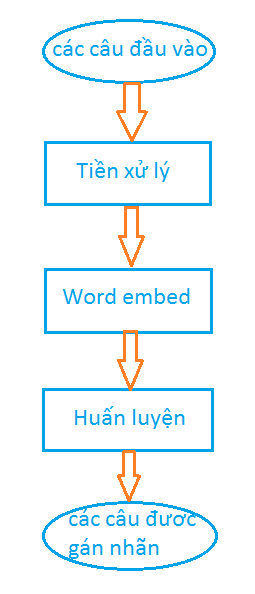
\includegraphics[width=0.35\textwidth]{model}
	  \captionof{figure}{Mô hình xử lý}  
	  \label{model}
	\end{center} 
\section{Tiền xử lý}
Quá trình tiền xử lý như sau:
	\begin{itemize}[label = \textbullet]
		\item Loại bỏ các kí tự không nằm trong bảng chữ cái
		\item Loại bỏ từ dừng
		\item Xây dựng tập từ điển nhằm phục vụ quá trình mã hóa từ(Word embedding)
	\end{itemize}
Một câu văn đầu vào có thể chứa những kí tự không nằm trong bảng chữ cái, các kí tự này cần được loại bỏ để giảm độ dài câu văn đồng thời tránh học những thông tin không cần thiết. Tương tự với từ dừng, loại bỏ các từ này sẽ không ảnh hưởng đến ý nghĩa của câu. 

Xây dựng tập từ điển là công đoạn khá quan trọng, các từ xuất hiện trong các câu sau khi đã thực hiện việc loại bỏ kí tự thừa và từ dừng sẽ được đưa vào từ điển. Mỗi từ sẽ ứng với một vị trí duy nhất trong từ điển. Các từ sẽ được mã hóa thành vector tương ứng sẽ được trình bày ở phần tiếp theo. 

Để thực hiện qúa trình tiền xử lý này chúng em sử dụng thư viện nltk, một công cụ mạnh mẽ được sử dụng trong xử lý ngôn ngữ tự nhiên

\section{Word Embedding}
Một vấn đề quan trọng trong xử lý ngôn ngữ tự nhiên là làm thể nào để máy tính có thể hiểu được ngôn ngữ của con người? Mã hóa từ (Word embedding) là một kỹ thuật giúp máy tính tiếp cận một cách dễ dàng với ngôn ngữ tự nhiên của chúng ta. Các từ sẽ được mã hóa bởi các vector tương ứng.

Về cơ bản, đây chỉ là một vector trọng số. Ví dụ, 1-of-N (one-hot vector) sẽ mã hoá (encoding) các từ trong từ điển thành một vector có chiều dài N (tổng số lượng các từ trong từ điển). Trong đó, có một phần tử mang giá trị 1 tương ứng với thứ tự của từ đó trong từ điển (ta có thể sắp từ điển tăng dần a-z, A-Z, 0-9) và các phần tử khác đều mang giá trị 0. Giả sử từ điển của chúng ta chỉ có 5 từ: King, Queen, Man, Woman, và Child. Ta có thể biểu diễn từ “Queen” như bên dưới:
	\begin{center}
	  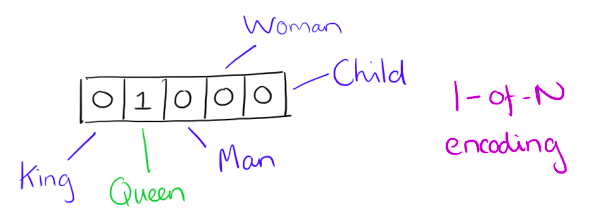
\includegraphics[width=0.7\textwidth]{one-hot}
	  \captionof{figure}{One-hot encoding}  
	  \label{one-hot}
	\end{center} 
Với cách mã hoá đơn giản như vậy, ta không thu được nhiều ý nghĩa trong việc so sánh các từ với nhau ngoại trừ so sánh bằng. Mặt khác, nếu kích thước từ điển quá lớn vì việc biểu diễn sẽ vô cùng lãng phí.
Word2vec được tìm ra để giải quyết các vấn đề này. Kỹ thuật này giúp chúng ta biểu diễn các từ bởi 1 vector có kích thước nhỏ hơn rất nhiều so với kích thước từ điển và các từ có quan hệ với nhau sẽ được biểu diễn bởi những vector gần nhau. Ví dụ chúng ta có 2 câu:
	\begin{itemize}[label = \textbullet]
		\item The kitten jumps over table
		\item This cat hunts mice
	\end{itemize}
Từ "kitten" và "cat" đều có nghĩa là "con mèo", vậy chúng cần được biểu diễn bởi 2 vector gần nhau
	\begin{center}
	  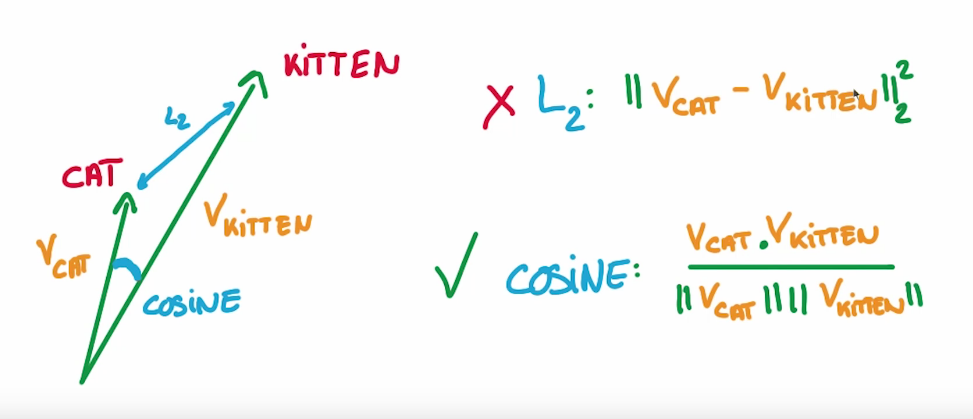
\includegraphics[width=0.7\textwidth]{cat}
	  \captionof{figure}{Khoảng cách giữa 2 vector}  
	  \label{cosin}
	\end{center} 
Độ đo $Cosin$ sẽ được sử dụng để xác định khoảng cách giữa 2 vector thay vì khoảng cách $Euclid$. Và để có thể tìm ra cách biểu diễn cho các từ, chúng ta cần sử dụng một mô hình học như: $Bag$ $of$ $words$, $Skip-gram$.

Trong nội dụng bài tập lớn, chúng em sẽ áp dụng mô hình $Skip-gram$ và sẽ được trình bày ở phần tiếp theo.
\subsection{The Skip-gram model}
Xét câu ví dụ sau:
	\begin{center}
	  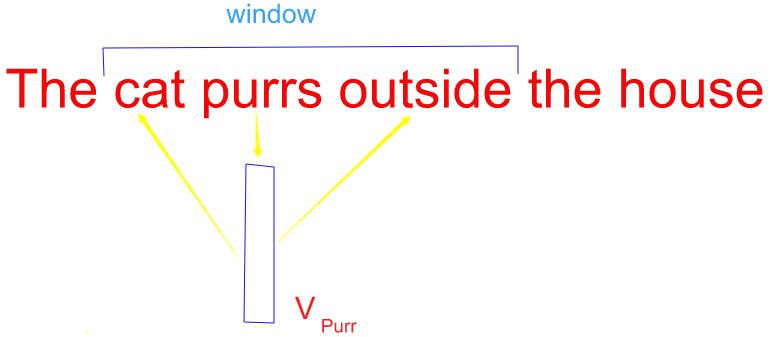
\includegraphics[width=0.7\textwidth]{sentence}
	  \captionof{figure}{Câu đầu vào}  
	  \label{sentence}
	\end{center} 
Đầu tiên, chúng ta sẽ chuẩn hóa các câu thành các các từ (target) và ngữ cảnh (context) mà nó xuất hiện trong đó. Định nghĩa $Ngữ$ $cảnh$ (context) bao gồm những từ bên trái và bên phải của từ target. Với kích thước của sổ bằng 1, ta thu được tập dữ liệu mới là các cặp (context, target) từ cầu đầu vào như sau:
	\begin{itemize}[label = \textbullet]
		\item (the, cat), (purr, cat), (cat, purr), (outside, purr)...
	\end{itemize} 
Công việc còn lại là tiến hành dự đoán $context$ từ $target$ tương ứng
	\begin{center}
	  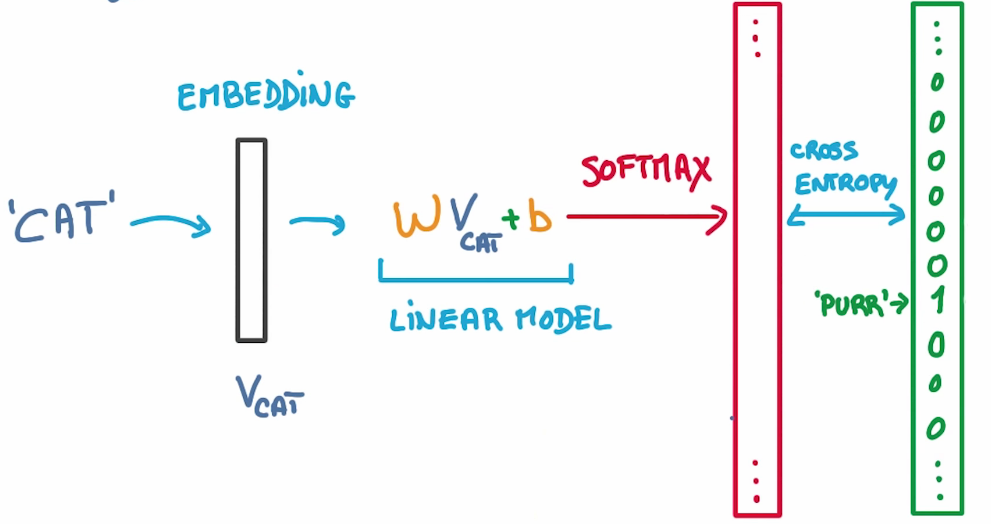
\includegraphics[width=0.7\textwidth]{skip-gram}
	  \captionof{figure}{The skip-gram model}  
	  \label{skip-gram}
	\end{center} 
Với một từ đầu vào, ta biểu diễn từ bởi một vector ngẫu nhiên $v \in R^{D}$, cho vector đi qua mô hình tuyến tính với 2 tham số $(W, b)$ và kết quả đầu ra thu được bởi hàm $softmax$. Mô hình cần tối ưu các tham số $v, w, b$ để cực tiểu hàm mục tiêu
	\begin{center}
		$C = -\frac{1}{n} \sum\limits_{x}{[ylna + (1-y)ln(1-a)]}$ \\
		
	\end{center}
	Trong đó:
		\begin{itemize}[label = \textbullet]
			\item a là vector đầu ra của mô hình
			\item y là kết quả thực tế, biểu diễn $context$ bởi vector one-hot encoding
		\end{itemize}
Quá trình tối ưu được thực hiện bằng ký thuật $Stochastic gradient descent$. Sau quá trình này, mỗi từ trong tử điển sẽ được biểu diễn bởi các vector tương ứng học được từ mô hình. Sau khi biểu diễn các từ bởi các vector, dữ liệu sẽ được đưa vào quá trình huấn luyện để xác định quan điểm cho từng câu đầu vào. Để thực hiện điều này, chúng ta sẽ sử dụng $Recurrent Neural Networks$
\section{Recurrent Neural Networks}
Recurrent Neural Networks (RNNs) là một trong những mô hình Deep learning được đánh giá có nhiều ưu điểm trong các tác vụ xử lý ngôn ngữ tự nhiên (NLP). Ý tưởng của RNNs đó là thiết kế một Neural Network sao cho có khả năng xử lý được thông tin dạng chuỗi (sequential information), ví dụ một câu là một chuỗi gồm nhiều từ. Recurrent có nghĩa là thực hiện lặp lại cùng một tác vụ cho mỗi thành phần trong chuỗi. Trong đó, kết quả đầu ra tại thời điểm hiện tại phụ thuộc vào kết quả tính toán của các thành phần ở những thời điểm trước đó.

Nói cách khác, RNNs là một mô hình có trí nhớ (memory), có khả năng nhớ được thông tin đã tính toán trước đó. Không như các mô hình Neural Network truyền thống đó là thông tin đầu vào (input) hoàn toàn độc lập với thông tin đầu ra (output). Về lý thuyết, RNNs có thể nhớ được thông tin của chuỗi có chiều dài bất kì, nhưng trong thực tế mô hình này chỉ nhớ được thông tin ở vài bước trước đó. Để có khả năng lưu trữ dài hạn, cần có một số cải tiến trong mỗi $cell$ $RNN$ và được thể hiện cụ thể trong mô hình $Long$ $short$ $term$ $memory$
	 
\subsection{Mạng RNN truyền thống}
	Dưới đây là mô hình Recurrent neural networks truyền thống
	\begin{center}
	  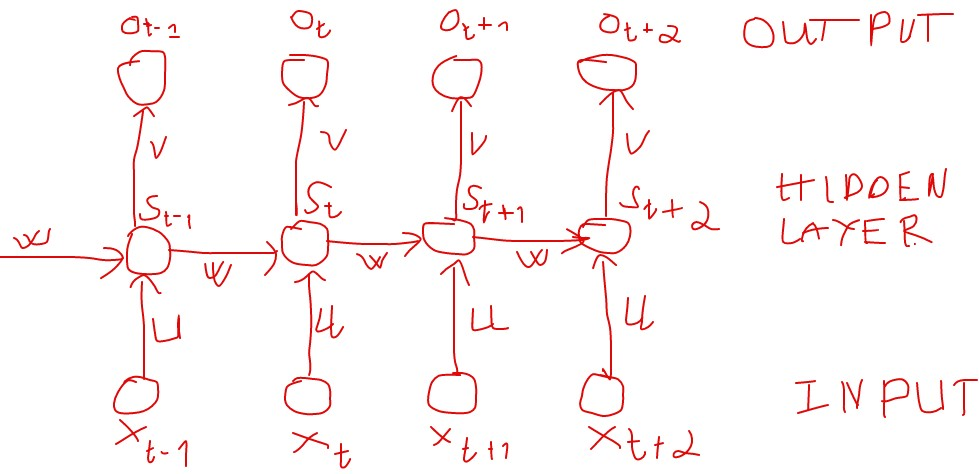
\includegraphics[width=0.7\textwidth]{RNN1}
	  \captionof{figure}{Kiến trúc Recurrent neural networks truyền thống}  
	  \label{RNNS1}
	\end{center}
	\begin{itemize}[label = \textbullet]
		\item $X_{t}$ là input tại thời điểm t.
		\item $S_{t}$ là trạng thái ẩn (memory) tại thời điểm t.
		\begin{center}
			$S_{t} = f(UX_{t} + S_{t-1}W)$, f là hàm tanh hoặc Relu.\\
			$tanh(x) = \frac{e^{x} - e^{-x}}{e^{x} + e^{-x}}$, $Relu(x) = max(x, 0)$
		\end{center}
		\item $O_{t}$ là output tại thời điểm t, $O_{t} = softmax(VS_{t})$
	\end{itemize}
Các tham số $U, W, V$ cần được tối ưu để cực tiểu hàm mục tiêu
	\begin{center}
			$C = E(y_{t}, \hat{y}_{t}) = - \sum\limits_{t}{y_{t}log(\hat{y}_{t})}$
	\end{center}
Huấn luyện RNNs tương tự như huấn luyện Neural Network truyền thống. Ta cũng sử dụng đến thuật toán backpropagation (lan truyền ngược) nhưng có một chút tinh chỉnh. Gradient tại mỗi output không chỉ phụ thuộc vào kết quả tính toán của bước hiện tại mà còn phụ thuộc vào kết quả tính toán của các bước trước đó. 

Cụ thể để tính Gradient của hàm mục tiêu đối với các tham số $W, U, V$ ta sẽ thuật toán Backpropagation through time với các công thức như sau:
		\begin{itemize}[label = \textendash]
			\item $\frac{\partial E_{t}}{\partial V} = (\hat{y}_{t} - y_{t}) \otimes S_{t}$
			\item $\frac{\partial E_t}{\partial W} = \sum\limits_{k=0}^{t} \frac{\partial E_t}{\partial \hat{y}_t}\frac{\partial\hat{y}_t}{\partial s_t}\frac{\partial s_t}{\partial s_k}\frac{\partial s_k}{\partial W}$
			\item $\frac{\partial E_t}{\partial U} = \sum\limits_{k=0}^{t} \frac{\partial E_t}{\partial \hat{y}_t}\frac{\partial\hat{y}_t}{\partial s_t}\frac{\partial s_t}{\partial s_k}\frac{\partial s_k}{\partial U}$
		\end{itemize}
Như đã trình bày ở trên, mạng $RNNs$ truyền thống không có khả năng nhớ dài hạn, vấn đề này sẽ ảnh hưởng rất lớn đến kết quả của việc phân loại trong trường hợp các câu quá dài. Vấn đề này được gọi là $vanishing$ $gradient$ (biến mất gradient).
	\begin{center}
	  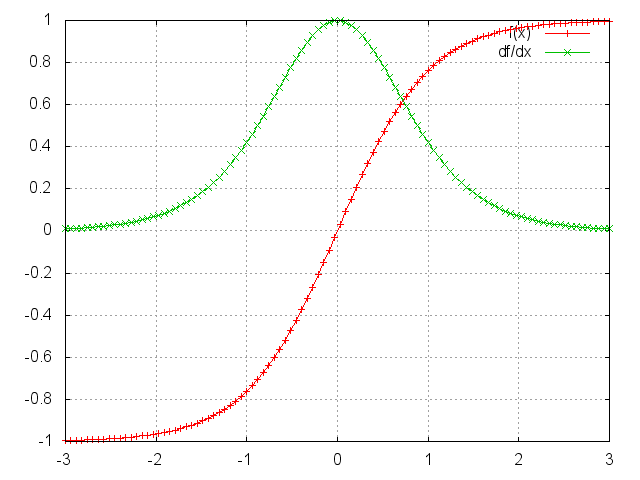
\includegraphics[width=0.7\textwidth]{tanh}
	  \captionof{figure}{Đồ thị biểu diễn đạo hàm của hàm tanh}  
	  \label{tanh}
	\end{center}
Trong công thức tính trạng thái ẩn $S_{t} = tanh(UX_{t} + S_{t-1}W)$, $S_{t}$ được biến đổi bởi hàm $tanh$. Nhìn vào đồ thị, ta dễ thấy Gradient của hàm $tanh$ luôn nằm trong khoảng (0, 1). Măt khác
	\begin{center}
		$\frac{\partial E_t}{\partial W} = \sum\limits_{k=0}^{t} \frac{\partial E_t}{\partial \hat{y}_t}\frac{\partial\hat{y}_t}{\partial s_t}\frac{\partial s_t}{\partial s_k}\frac{\partial s_k}{\partial W}=\sum\limits_{k=0}^{t} \frac{\partial E_t}{\partial \hat{y}_t}\frac{\partial\hat{y}_t}{\partial s_t} \left(\prod\limits_{j=k+1}^{t} \frac{\partial s_j}{\partial s_{j-1}}\right) \frac{\partial s_k}{\partial W}$\\
		$\Rightarrow \prod\limits_{j=k+1}^{t} \frac{\partial s_j}{\partial s_{j-1}}$ sẽ tiến tới 0 nếu độ dài câu quá dài. 
	\end{center}
Vấn đề này sẽ dẫn đến việc huấn luyện sẽ bị dừng lại. $Long$ $short$ $term$ $memory$ sẽ giải quyết vấn đề này.

\subsection{Long short term memory}
Mô hình này có cấu trúc tương tự như RNNs nhưng có cách tính toán khác đối với các hidden state. Memory trong LSTMs được gọi là cells (hạt nhân). Ta có thể xem đây là một hộp đen nhận thông tin đầu vào gồm hidden state $s_{t-1}$ và giá trị $x_t$. Bên trong các hạt nhân này, chúng sẽ quyết định thông tin nào cần lưu lại và thông tin nào cần xóa đi, nhờ vậy mà mô hình này có thể lưu trữ được thông tin dài hạn.
	\begin{center}
	  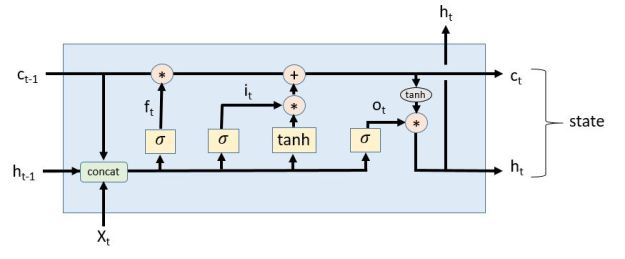
\includegraphics[width=0.8\textwidth]{lstm}
	  \captionof{figure}{Kiến trúc cell LSTMs}  
	  \label{lstm}
	\end{center}
Các biến đổi trong cells cụ thể như sau:
	\begin{itemize}[label = \textbullet]
		\item $i = \sigma(X_tU^i + S_{t-1}W^i)$
		\item $f = \sigma(X_tU^f + S_{t-1}W^f)$ 
		\item $o = \sigma(X_tU^o + S_{t-1}W^o)$
		\item $g = tanh(X_tU^g + S_{t-1}W^g)$
		\item $C_t = C_{t-1} \otimes f + g \otimes o$
		\item $S_t = o \otimes tanh(C_t)$
	\end{itemize}
Ba cổng input, output, forget sẽ quyết định bao nhiêu lượng thông tin sẽ nên được lưu giữ lại. 
	\begin{itemize}[label = \textbullet]
		\item Cổng input xác định bao nhiêu lượng thông tin tại trạng thái hiện tại sẽ được lưu giữ
		\item Cổng forget xác định bao nhiêu lượng thông tin trong quá khứ sẽ được giữ lại
		\item Cổng output xác định bao nhiêu lượng thông tin tính đến thời điểm hiện tại sẽ được truyền đi tới nơ-ron tiếp theo
	\end{itemize} 
Mô hình này là một bước đột phá mà chúng ta đạt được từ mô hình RNNs và có thể trong tương lai chúng ta sẽ tim ra được những mô hình tốt hơn.

Dưới đây là mô hình cụ thể mà chúng em sử dụng trong bài toán phân tích quan điểm: 
	\begin{center}
	  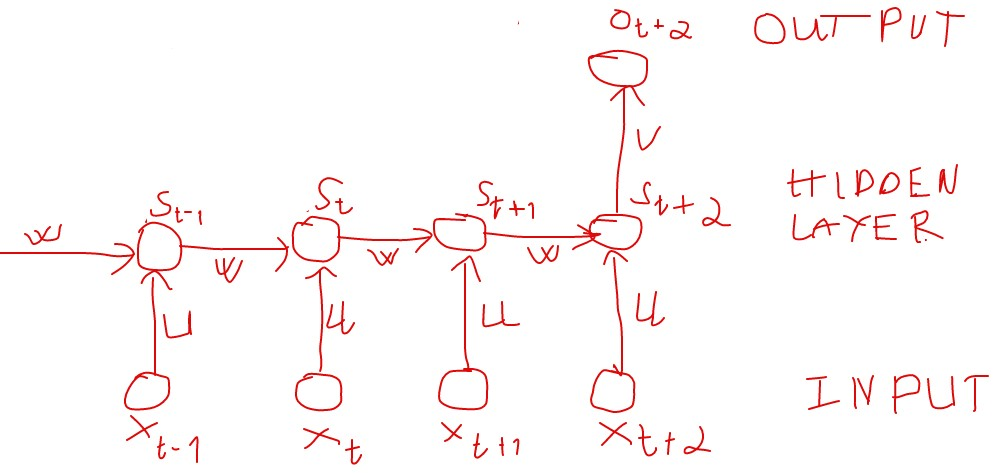
\includegraphics[width=0.8\textwidth]{RNN2}
	  \captionof{figure}{Mô hình sử dụng}  
	  \label{rnns2}
	\end{center}
	\begin{itemize}[label = \textbullet]
		\item $X_t$ là từ thứ t trong câu
		\item output là vector duy nhất $O \in R ^{D}$
		\begin{itemize}[label = \textendash]
			\item $D = 2$ trong trường hợp binary-class
			\item $D = 5$ trong trường hợp multi-class
		\end{itemize} 		
	\end{itemize}